\section{Fundamentação teórica}

De acordo com o postulado 1 de Bohr, os elétrons se movem numa órbita eliptica (assumida circular)
em torno do núcleo, sob influência da força de Coulomb. 
Temos então
\begin{equation}
F = \frac{kZe^2}{r^2} = \frac{mv^2}{r} 
\implies v = \left( \frac{kZe^2}{mr} \right)^{1/2}  \;.
\end{equation}

\noindent Pelo postulado 2, temos
\begin{equation}
L = mvr = n\hbar, \quad n \in \mathbb{N} \;.
\end{equation}

\noindent Substituindo a expressão para $v$ obtida anteriormente, e explicitando $r$, obtemos
\begin{equation}
r_n = \frac{n^2 \hbar^2}{mkZe^2} \;.
\label{eq: bohr radius}
\end{equation}

\noindent A energia total do elétron é 
\begin{equation}
E = \frac{mv^2}{2} + V(r) = \frac{kZe^2}{2r} - \frac{kZe^2}{r} = -\frac{kZe^2}{2r} \;.
\label{eq: atom energy}
\end{equation}

\noindent Substituindo a Eq. \eqref{eq: bohr radius} na \eqref{eq: atom energy}, obtemos que
\begin{equation}
E_n = -E_0 \frac{Z^2}{n^2}, \quad E_0 \equiv \frac{mk^2e^4}{e\hbar^2} \;.
\end{equation}

Os postulados de Bohr implicam então que a energia das órbitas estacionárias é quantizada. 
Assim, as energias a que o postulado 4 se refere devem pertencer ao conjunto de energias permitidas. \cite{tipler}

Embora diversas aproximações tenham sido feitas para derivar essas expressões, como assumir que as órbitas são
circulares, as previsões concordam com os resultados empíricos. 
No entanto, quanto maior o número atômico, maior é a disparidade entre as previsões do modelo de Bohr e as 
medidas em laboratório. 
Mesmo os valores numéricos sendo diferentes, continua sendo fato inegável que a energia dos átomos é quantizada, 
e apenas é possível levar um átomo em um estado de menor energia para um de maior se for fornecida a quantidade 
exata necessária para isso. 

Em 1914, apenas um ano após a publicação do trabalho de Bohr, Franck e Hertz realizaram um experimento que comprovou a
quantização da energia dos átomos, cujo esquema está mostrado na Fig. \ref{fig: esquema franckhertz}. 

\begin{figure}[h]
\centering
\caption{Esquema do equipamento utilizado por Franck e Hertz em seu famoso experimento.}
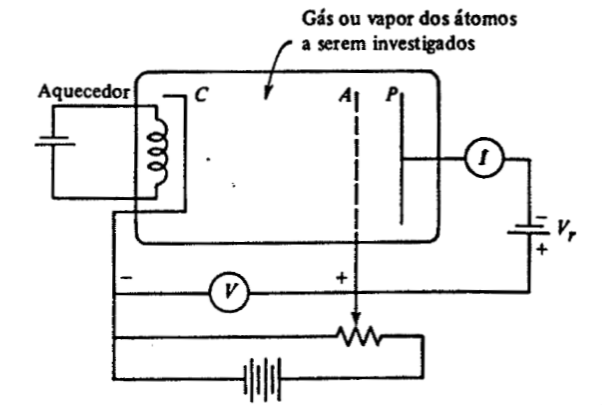
\includegraphics[width=.95\linewidth]{imagens/esquema_franckhertz.png}
\small{\\Fonte: \cite{eisberg}.}
\label{fig: esquema franckhertz}
\end{figure}

Dentro de um tubo selado, um cátodo aquecido $C$ emite termicamente elétrons de baixa energia. 
Eles são acelerados por um potencial de excitação $V$ em direção a um ânodo $A$.
Alguns elétrons atravessam $A$ e chegam até uma placa coletora $P$, desde que sua energia cinética ao 
atravessar $A$ seja suficiente para vencer um pequeno potencial de retardo $V_r$ aplicado entre $P$ e $A$. 
Um amperímetro mede a corrente de retorno $I$ que vem de $P$, que é uma medida da quantidade de elétrons que chegam à placa.

Seja $T$ a temperatura próximo a $C$. 
Para $T$ e $V_r$ fixos, a medida que $V$ cresce, a energia cinética média dos elétrons ao atravessar 
o anoto também cresce, e portanto mais elétrons devem alcançar $P$.
Assim, é esperado que $I$ aumente com $V$. 

Dentro do tubo há também algum gás monoatômico.
Os elétrons acelerados então possuem uma chance de colidir com algum dos átomos, que se encontram no estado fundamental. 
No entanto, se a energia cinética do elétron for menor que a energia $\Delta$ necessaria para levar o átomo para o primeiro
estado excitado, a colisão é perfeitamente elástica, e não há perda de energia por parte do elétron.

No entanto, quando $V$ for exatamente igual a $\Delta$, os átomos mais energéticos 
que são ejetados de $C$ podem realizar colisões inelásticas com os átomos, fazendo com que não mais consigam 
superar o potencial de retardo. 
A medida que $V$ aumenta após esse valor crítico, uma porcentagem cada vez maior dos elétrons ejetados passa a 
poder realizar colisões inelásticas, fazendo $I$ se tornar uma função decrescente de $V$. 

Aumentando $V$ ainda mais, mesmo os elétrons que perderam energia para os átomos são acelerados o suficiente para que
cheguem em $P$, e assim $I$ torna a aumentar com $V$. 
Quando $V$ for $2\Delta$, mesmo um elétron que já transferiu sua energia uma vez pode acabar realizando uma segunda 
transferência, ocasionando um segundo máximo de $I$ em função de $V$. 

Continuando essa lógica, é possível concluir que para $V = n\Delta$, $n \in \mathbb{N}$, $I(V)$ possui um máximo local,
comportamento que só pode ser explicado pela quantização da energia dos átomos. 

Considere agora que o processo é repetido para diferentes valores de $T$, fixado $V_r$. 
Um $T$ maior implica que a distribuição das velocidades dos elétrons ao sair do cátodo possui uma largura maior. 
Também aumenta a pressão do gás dentro do tubo, tornando as colisões mais frequentes.
Com efeito, se a temperatura for suficientemente baixa, espera-se não ser possível observar o os máximos de $I(V)$, pois 
colisões de elétrons com átomos se tornam extremamente improváveis.
Esses dois efeitos combinados indicam que ao aumentar a temperatura no cátodo, a curva de $I(V)$ será mais 
suave e será possível observar mais máximos de corrente, embora cada máximo permaneça no mesmo valor de $V$.

Considere agora que é fixado $T$, e o gráfico de $I$ por $V$ é construido para diferentes valores de $V_r$. 
O efeito esperado ao aumentar o potencial de retardo é que os valores numéricos de $I$ sofram uma queda global, 
pois o anodo passa a causar uma repulsão maior nos elétrons. 
No entanto, a probabilidade de um elétron transferir ou não energia para um átomo durante o percurso de $C$ a $A$ é independente de $V_r$, 
portanto é esperado também que os picos permaneçam no mesmo lugar. \cite{eisberg} \cite{tipler} \cite{roteiro}
